\documentclass{article}
\usepackage{cmap}
\usepackage[utf8]{inputenc}
\usepackage[english,ukrainian]{babel}
\usepackage{graphicx}
\usepackage{geometry}
\usepackage{listings}
\usepackage{float}
\usepackage{amsmath}
\geometry{
	a4paper,
	left=20mm,
	right=20mm,
	top=15mm,
	bottom=15mm,
}
\lstset{
	language=c,
	tabsize=4,
	keepspaces,
	showstringspaces=false,
}
\graphicspath{ {./pictures} }
\setlength{\parindent}{4em}

\newcommand\subject{Організація комп’ютерних мереж}
\newcommand\lecturer{асистент кафедри ПЗ \\ Задорожний І.М.}
\newcommand\teacher{асистент кафедри ПЗ \\ Задорожний І.М.}
\newcommand\mygroup{ПЗ-22}
\newcommand\lab{3}
\newcommand\theme{Дослідження та робота з таблицею маршрутизації у Windows XP}
\newcommand\purpose{Ознайомитися з принципами маршрутизації та навчитися користуватися утилітою route для зміни таблиці маршрутизації вручну}

\begin{document}
\begin{normalsize}
	\begin{titlepage}
		\thispagestyle{empty}
		\begin{center}
			\textbf{МІНІСТЕРСТВО ОСВІТИ І НАУКИ УКРАЇНИ\\
				НАЦІОНАЛЬНИЙ УНІВЕРСИТЕТ "ЛЬВІВСЬКА ПОЛІТЕХНІКА"}
		\end{center}
		\begin{flushright}
			\textbf{ІКНІ}\\
			Кафедра \textbf{ПЗ}
		\end{flushright}
		\vspace{200pt}
		\begin{center}
			\textbf{ЗВІТ}\\
			\vspace{10pt}
			до лабораторної роботи № \lab\\
			\textbf{на тему}: “\textit{\theme}”\\
			\textbf{з дисципліни}: “\subject”
		\end{center}
		\vspace{112pt}
		\begin{flushright}
			
			\textbf{Лектор}:\\
			\lecturer\\
			\vspace{28pt}
			\textbf{Виконав}:\\
			
			студент групи \mygroup\\
			Коваленко Д.М.\\
			\vspace{28pt}
			\textbf{Прийняв}:\\
			
			\teacher\\
			
			\vspace{28pt}
			«\rule{1cm}{0.15mm}» \rule{1.5cm}{0.15mm} 2023 р.\\
			$\sum$ = \rule{1cm}{0.15mm}……………\\
			
		\end{flushright}
		\vspace{\fill}
		\begin{center}
			\textbf{Львів — 2023}
		\end{center}
	\end{titlepage}
		
	\begin{description}
		\item[Тема.] \theme.
		\item[Мета.] \purpose.
	\end{description}

\section*{Теоретичні відомості}
\begin{enumerate}
	\item[2.] Де застосовується маршрутизація за попереднім досвідом?
	Маршрутизація за попереднім досвідом (англ. "Policy-based routing" або "PBR") - це технологія маршрутизації, яка дозволяє визначати маршрутизаційні правила на основі певних параметрів, таких як IP-адреси, порти, протоколи, тощо.
	
	Основне застосування маршрутизації за попереднім досвідом полягає в тому, щоб дозволити мережевим адміністраторам керувати трафіком мережі та забезпечити оптимальний шлях для різних типів даних. Наприклад, можна встановити правила маршрутизації для надання переваги трафіку з певного джерела, для використання альтернативних маршрутів або для обмеження швидкості трафіку. 
\end{enumerate}

\section*{Хід виконання}
 
\begin{figure}[H]
	\centering
	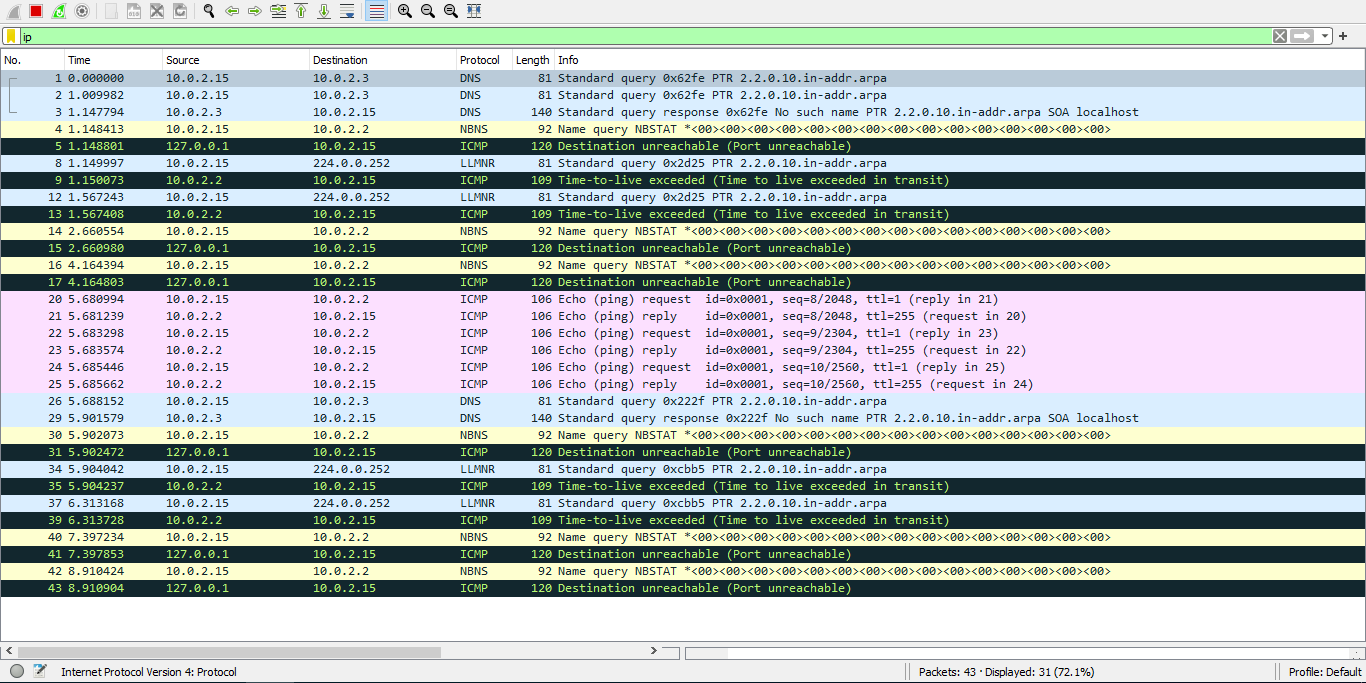
\includegraphics[width=\textwidth]{11}
	\caption{Пакети відправлені на адресу маршрутизатора при виконанні команди tracert}
\end{figure}

\begin{figure}[H]
	\centering
	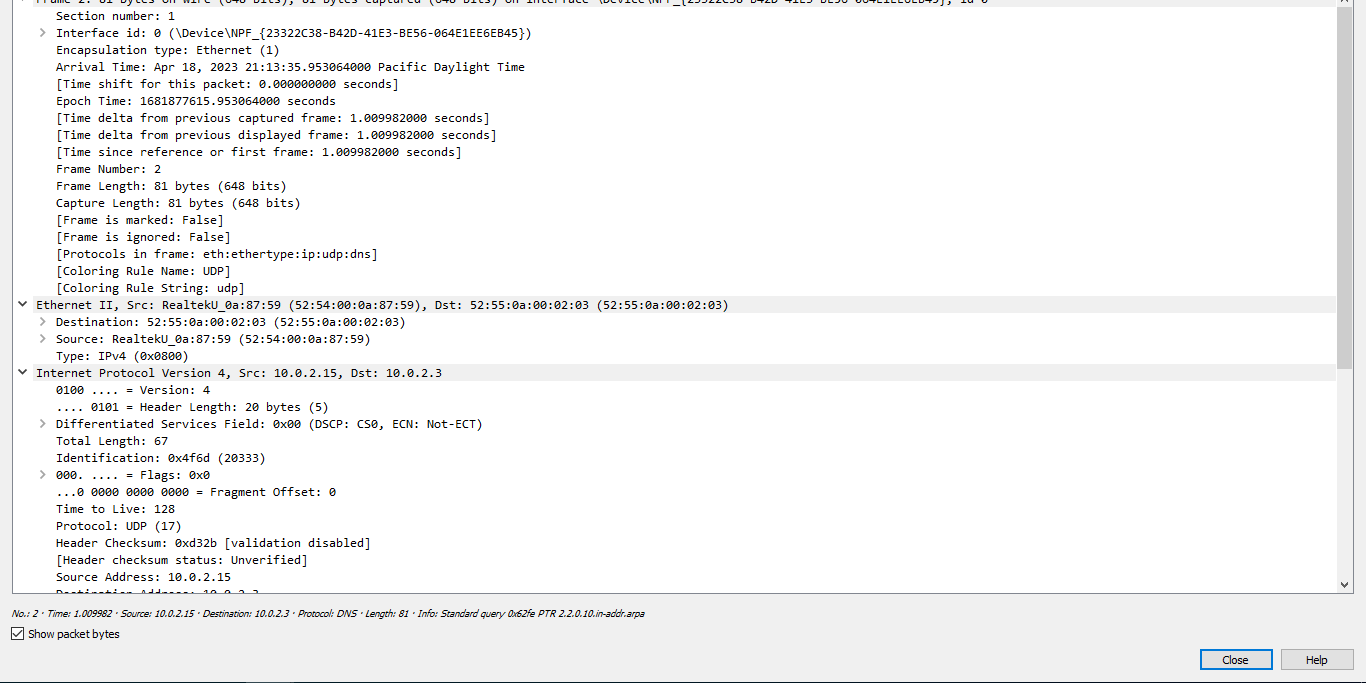
\includegraphics[width=\textwidth]{12}
	\caption{Вміст одного з пакетів відправлених на адресу маршрутизатора 1/2}
\end{figure}

\begin{figure}[H]
	\centering
	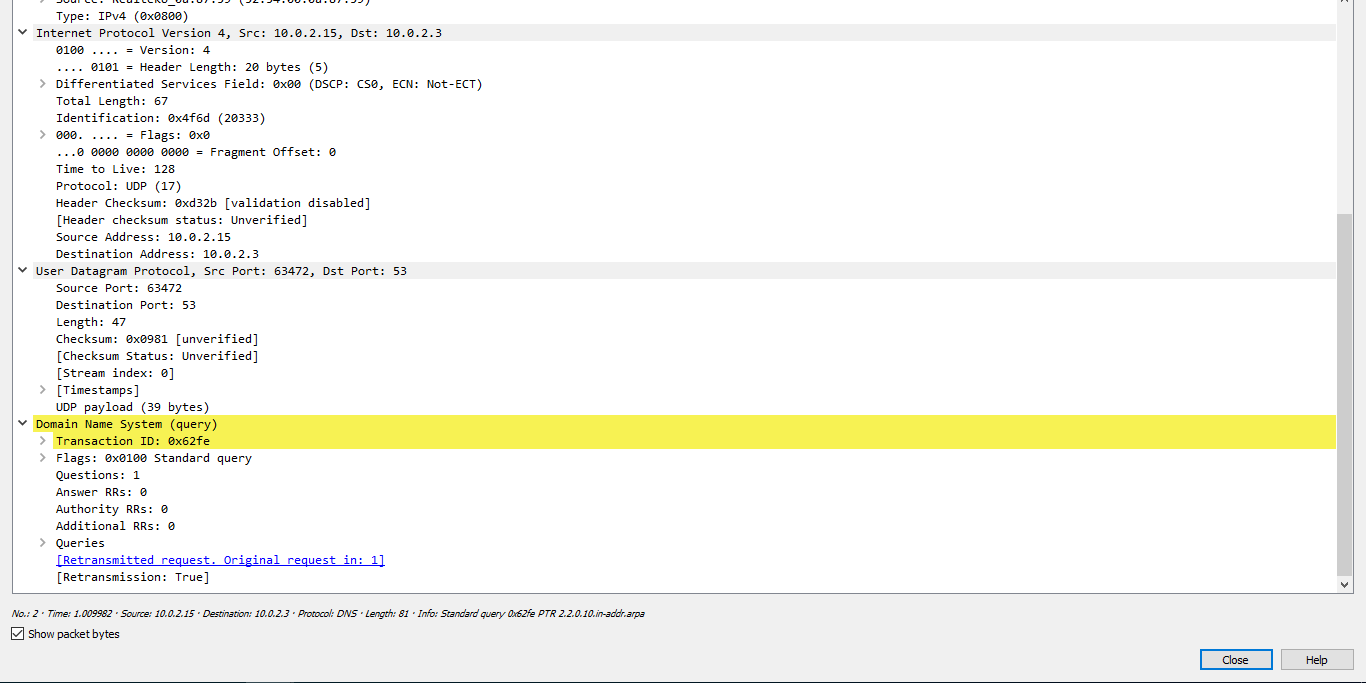
\includegraphics[width=\textwidth]{13}
	\caption{Вміст одного з пакетів відправлених на адресу маршрутизатора 2/2}
\end{figure}

Виходячи з IP-адреси мого комп'ютера (10.0.2.15) та маски підмережі (255.255.255.0) визначив (користуючись теоретичним матеріалом і наведеними прикладами в презентаціях у ВНС): адресу мережі (10.0.2.0), широкомовну адресу (10.0.2.255), адреси першого (10.0.2.1) і останнього вузлів (10.0.2.254), загальну кількість комп’ютерів в цій мережі (254).

\begin{figure}[H]
	\centering
	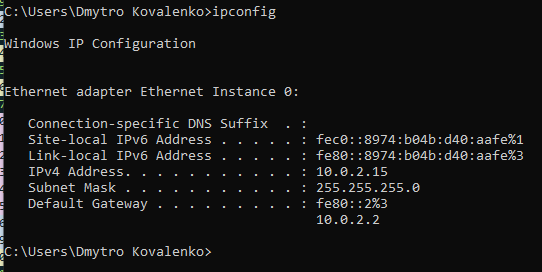
\includegraphics[width=\textwidth]{21}
	\caption{Виконання команди ipconfig}
\end{figure}

Проаналізував цю таблицю і визначив тип адрес (загальна, приватна, адреса мережі, вузла, багатоадресної або широкомовної розсилки).

\begin{figure}[H]
	\centering
	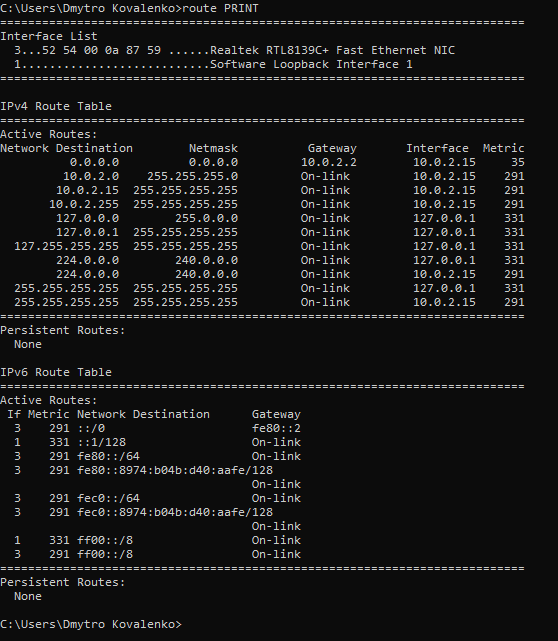
\includegraphics[width=\textwidth]{31}
	\caption{Виконання команди route з аргументом PRINT}
\end{figure}

\begin{list}{-}{}
	\item Адреса мережі 10.0.2.0 з маскою мережі 255.255.255.0 є приватною адресою, оскільки маска мережі вказує на діапазон приватних мереж.
	\item Адреса мережі 0.0.0.0 з маскою мережі 0.0.0.0 є маршрутом за замовчуванням, тобто цей маршрут використовується для пересилання всіх пакетів, які не мають специфічного маршруту.
	\item Адреси мережі 127.0.0.0, 127.0.0.1, 127.255.255.255 з маскою мережі 255.0.0.0 є адресами мережі тестового циклу (loopback address) і використовуються для зв'язку з мережею власного пристрою.
	\item Адреса мережі 224.0.0.0 з маскою мережі 240.0.0.0 є багатоадресною адресою, що використовується для розсилки пакетів на кілька адрес одночасно.
\end{list}

\begin{figure}[H]
	\centering
	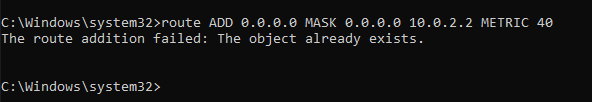
\includegraphics[width=\textwidth]{32}
	\caption{Виконання команди route з існуючою адресою шлюзу}
\end{figure}

\begin{figure}[H]
	\centering
	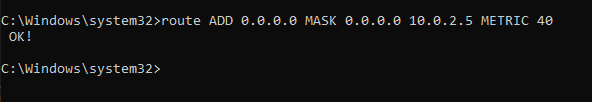
\includegraphics[width=\textwidth]{33}
	\caption{Виконання команди route ADD з неіснуючою адресою шлюзу}
\end{figure}

\begin{figure}[H]
	\centering
	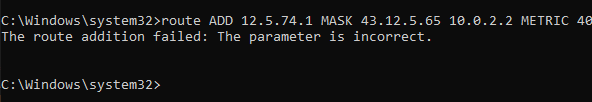
\includegraphics[width=\textwidth]{34}
	\caption{Виконання команди route ADD з випадковими значеннями вузла та маски}
\end{figure}

\begin{figure}[H]
	\centering
	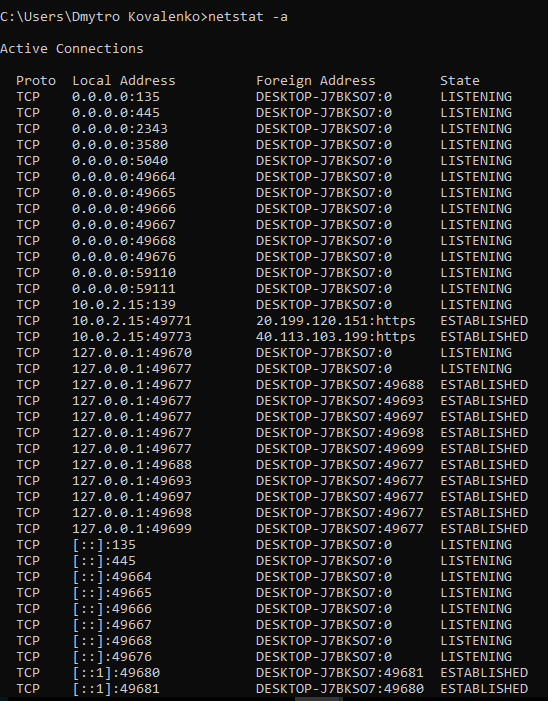
\includegraphics[width=\textwidth]{41}
	\caption{Визначив відкриті порти, протоколи, за якими виконані
		підключення комп'ютера 1/2}
\end{figure}

\begin{figure}[H]
	\centering
	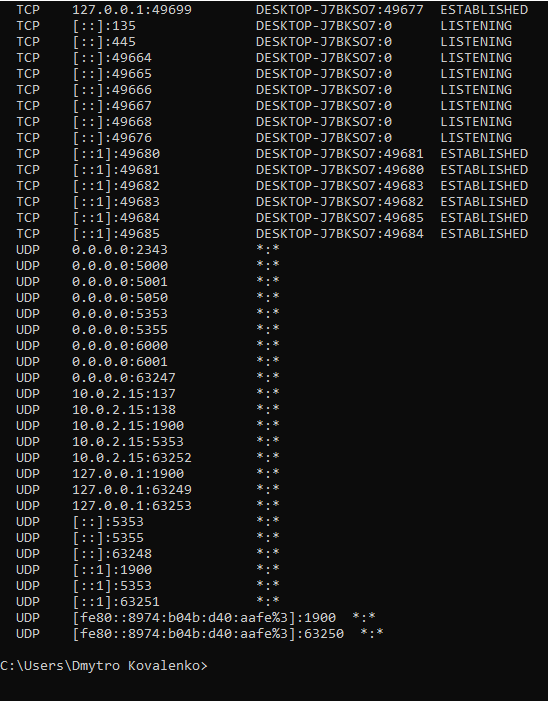
\includegraphics[width=\textwidth]{42}
	\caption{Визначив відкриті порти, протоколи, за якими виконані
		підключення комп'ютера 2/2}
\end{figure}

\begin{figure}[H]
	\centering
	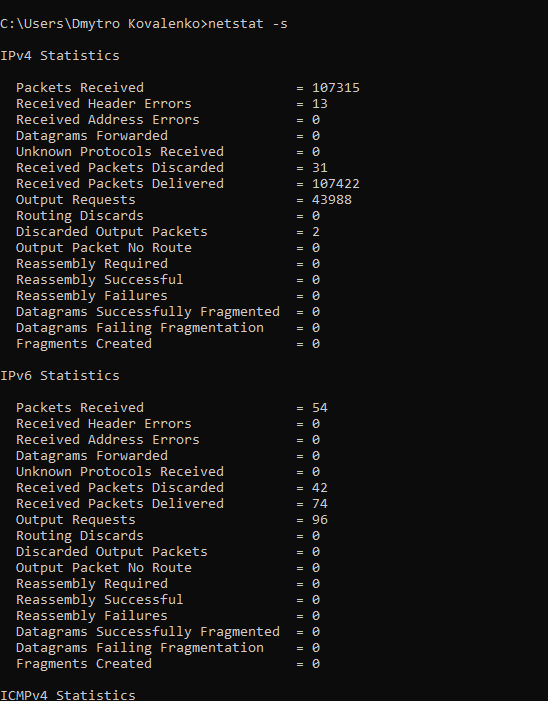
\includegraphics[width=\textwidth]{51}
	\caption{Статистичні дані про підключення
		мого комп'ютера 1/3}
\end{figure}

\begin{figure}[H]
	\centering
	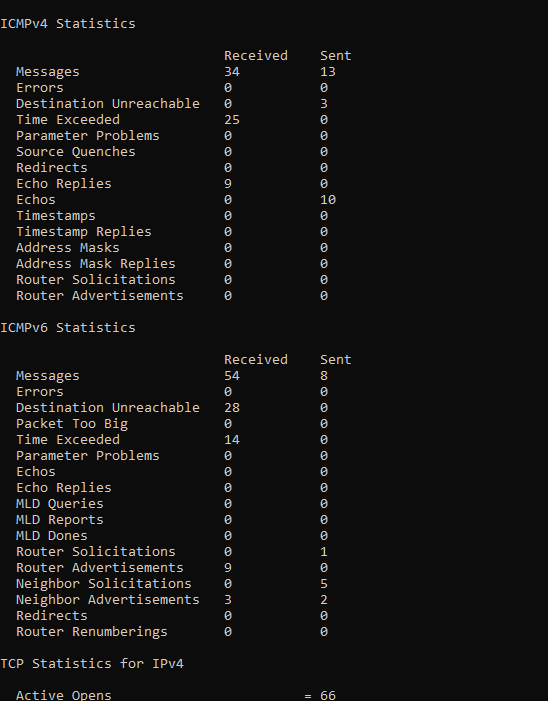
\includegraphics[width=\textwidth]{52}
	\caption{Статистичні дані про підключення
		мого комп'ютера 2/3}
\end{figure}

\begin{figure}[H]
	\centering
	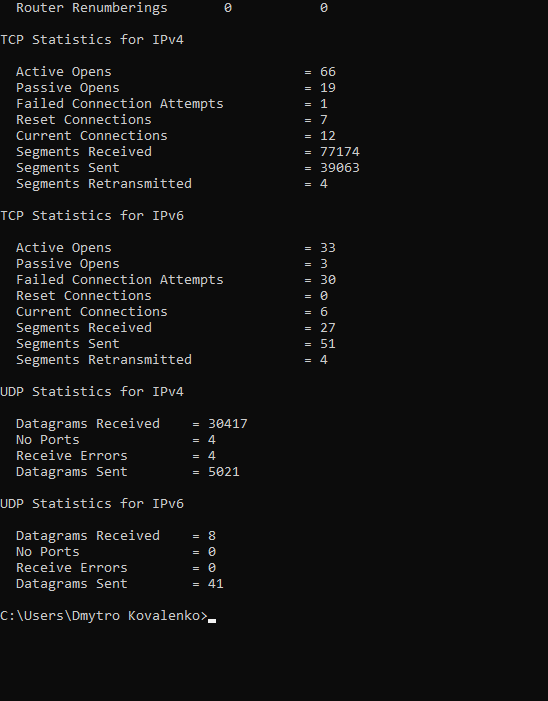
\includegraphics[width=\textwidth]{53}
	\caption{Статистичні дані про підключення
		мого комп'ютера 3/3}
\end{figure}

Самостійно знайшов детальну інформацію про призначення поля Інтерфейс у таблиці маршрутизації:

Поле "інтерфейс" в таблиці маршрутизації вказує на мережевий інтерфейс, через який потрібно проходити, щоб дістатися до мережі або IP-адреси, визначеної в полі "Destination". Це поле є дуже важливим, оскільки воно дозволяє визначити, який конкретний інтерфейс повинен використовуватися для передачі даних до конкретної мережі.

Наприклад, якщо в системі є два мережеві інтерфейси, один з'єднаний з Інтернетом, а інший - з локальною мережею, таблиця маршрутизації допоможе визначити, який інтерфейс потрібно використовувати для взаємодії з конкретною мережею. Відповідно, використання правильного мережевого інтерфейсу дозволить забезпечити оптимальну швидкість передачі даних та забезпечити безпеку мережі.

Самостійно знайшов інформацію про призначення протоколу IGMP і його зв'язок з протоколом ICMP

Протокол IGMP (Internet Group Management Protocol) використовується в мережах IP для керування групами мультикасту. Він дозволяє пристроям підписуватися на мультикастові групи та отримувати мультикастовий трафік, який передається в мережі.

Протокол ICMP (Internet Control Message Protocol) використовується в мережах IP для передачі повідомлень про помилки та інших станів мережі. ICMP використовується для передачі повідомлень про помилки в IP-пакетах, включаючи такі помилки, як недоступність мережі, недоступність хоста, TTL закінчився та інші.

Хоча IGMP та ICMP є протоколами різних рівнів мережевої моделі, вони пов'язані між собою. Конкретно, коли пристрій підписується на мультикастову групу за допомогою IGMP, він відправляє повідомлення IGMP-запиту на мультикастову адресу. Якщо інший пристрій вже є членом цієї групи, він може відправити повідомлення IGMP-відповіді, щоб повідомити першого пристрою про свою присутність в групі. Якщо пристрій не отримує відповіді від інших пристроїв, він може повторити запит, використовуючи протокол ICMP, щоб перевірити, чи доступний мережевий шлях до цієї мультикастової групи.

Отже, хоча IGMP і ICMP є різними протоколами, вони можуть взаємодіяти, щоб забезпечити оптимальну роботу мережі та надати користувачам доступ до мультикастового трафіку.
\section*{Висновки}
Під час виконання лабораторної роботи я ознайомився з принципами маршрутизації та навчився користуватися утилітою route для зміни таблиці маршрутизації вручну
	    
\end{normalsize}
\end{document}
